\chapter{Introducción a ROS}

\thispagestyle{plain}
\renewcommand{\tablename}{Tabla}

\section{Introducción}

Durante el desarrollo de este proyecto se planteó la posibilidad implementar ROS en el controlador. Para ello fue necesario familiarizarse con el funcionamiento de este \textit{middleware} robótico. 

\section{Software Adicional}
\subsection{VMware Workstation 17 Player}

VMware Workstation 17 Player es una aplicación de virtualización de escritorio desarrollada por VMware. Permite a los usuarios ejecutar múltiples sistemas operativos simultáneamente en una sola máquina física mediante la creación y gestión de máquinas virtuales.

\begin{figure}[H]
    \centering
    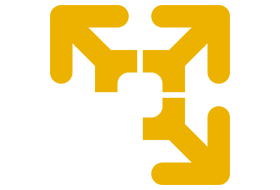
\includegraphics[width=0.25\linewidth]{imagenes/Logo VMware.png}
    \caption{Logotipo VMware \cite{VMware}}
\end{figure}

Este aplicación será la que se utilice, con el sistema operativo Ubuntu, para realizar las simulaciones de pruebas con ROS.

\subsubsection{Ubuntu}

Ubuntu es una distribución de Linux basada en Debian, desarrollada y mantenida por Canonical Ltd. Es conocida por su enfoque en la facilidad de uso, accesibilidad y regularidad en las actualizaciones lo que la convierte en una opción popular tanto para usuarios principiantes como para profesionales. Una de las características destacadas de Ubuntu es su compromiso con el software libre y de código abierto, permitiendo a los usuarios modificar y distribuir el sistema operativo según sus necesidades.

\begin{figure}[H]
    \centering
    
\includegraphics[width=0.25\linewidth]{imagenes/Logo Ubuntu.png}
    \caption{Logotipo Ubuntu \cite{Ubuntu}}
\end{figure}

Durante esta parte del proyecto, utilizaremos la versión de Ubuntu 20.04.6 LTS, proporcionada por MathWorks \cite{MatlabROSVirtual}. 

\begin{figure}[H]
    \centering
    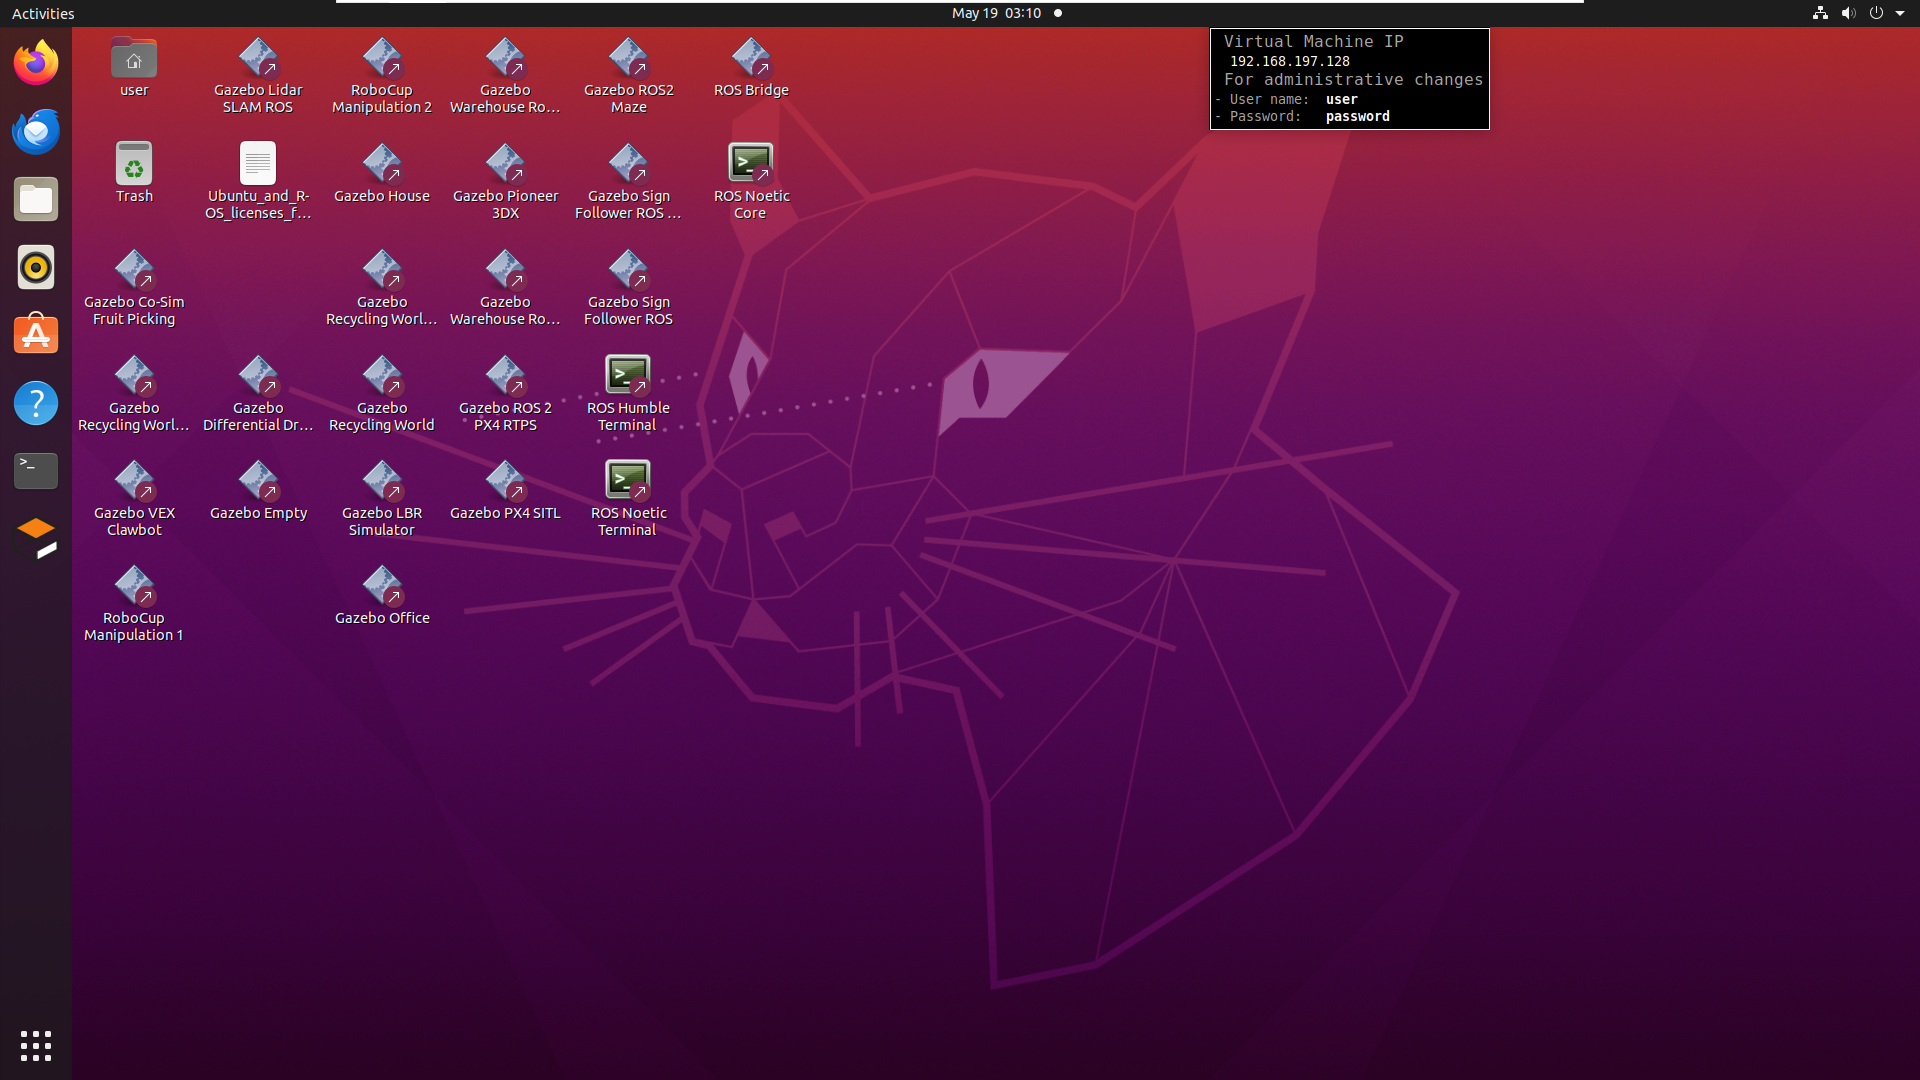
\includegraphics[width=0.75\linewidth]{imagenes/IntroROS - Vista Inicial Ubuntu.png}
    \caption{Escritorio de la máquina virtual ros\_noetic\_foxy\_gazebov11.vmx}
    \label{fig:enter-label}
\end{figure}

\subsubsection{Gazebo}

Gazebo es un simulador de robots en 3D de código abierto ampliamente utilizado en la investigación y desarrollo de robótica. Permite la simulación de sistemas robóticos complejos en un entorno visual realista, ofreciendo física avanzada, gráficos de alta calidad y una interfaz para interactuar con los robots. Gazebo es capaz de simular diversos sensores, actuadores y entornos, lo que facilita la prueba y validación de algoritmos y diseños de robots sin necesidad de hardware.

\begin{figure}[H]
    \centering
    
\includegraphics[width=0.25\linewidth]{imagenes/Logo Gazebo.png}
    \caption{Logotipo Gazebo \cite{Gazebo}}
\end{figure}

Este simulador permite su integración con ROS, es por ello por lo que se utiliza en esta parte del proyecto.

\section{Configuración}

Lo primero sería configurar la red, para ello se deben modificar dos variables del entorno ROS: ROS\_MASTER\_IP y ROS\_IP. Estas variables se suelen establecer automáticamente, pero se deben comprobar. Para ello se abre la terminal de Ubuntu (Ctrl+Alt+T) y se escriben los siguientes comandos:

\begin{lstlisting}[language=bash, caption=Comprobación variables]
ifconfig
echo $ROS_MASTER_URI
echo $ROS_IP
\end{lstlisting}

\begin{figure}[H]
    \centering
    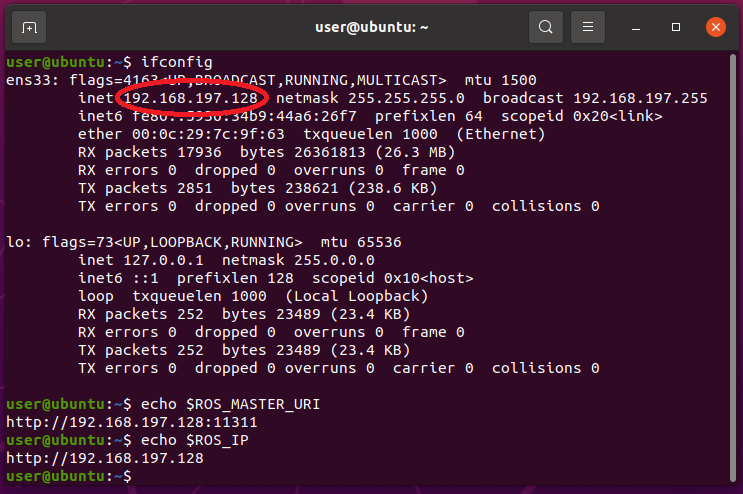
\includegraphics[width=0.75\linewidth]{imagenes/IntroROS - Configuracion Red.png}
    \caption{Configuración red.}
    \label{fig:Ubuntu - Configuracion Red}
\end{figure}

En caso de que estas IPs no coincidan, se deberán cambiar usando los siguientes comandos, sustituyendo `IP\_OF\_VM' con la IP que corresponde a la máquina virtual (Figura \ref{fig:Ubuntu - Configuracion Red}):

\begin{lstlisting}[language=bash, caption=Configuración variables]
echo export ROS_MASTER_URI=http://IP_OF_VM:11311 >> ~/.bashrc
echo export ROS_IP=IP_OF_VM >> ~/.bashrc
\end{lstlisting}

Para realizar esto es necesario que la máquina virtual tenga acceso a internet. En algunos casos se detectó que la máquina virtual no se conectaba automáticamente, para solucionar este problema, se ejecutan en terminal los siguientes comandos (sustituyendo `35' por el número correspondiente):

\begin{lstlisting}[language=bash, caption=Solución conexión a internet]
ifconfig -a
sudo dhclient ens35
\end{lstlisting}

El siguiente diagrama ilustra las asignaciones correctas de variables de entorno (con direcciones IP falsas)

\begin{figure}[H]
    \centering
    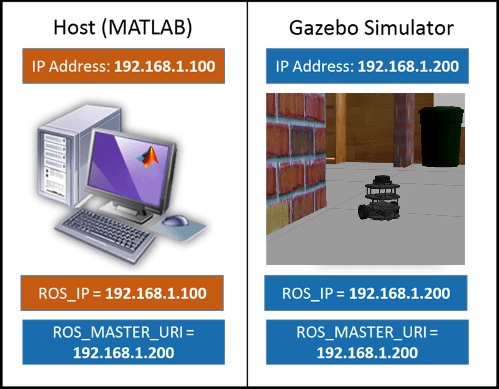
\includegraphics[width=0.5\linewidth]{imagenes/ROS - Mathworks.png}
    \caption{Diagrama de variables de entorno \cite{GazeboMatlab}}
    \label{fig:enter-label}
\end{figure}

Una vez configurada correctamente la red, se procede a abrir el ejemplo de `Gazebo House'.

\begin{figure}[H]
    \centering
    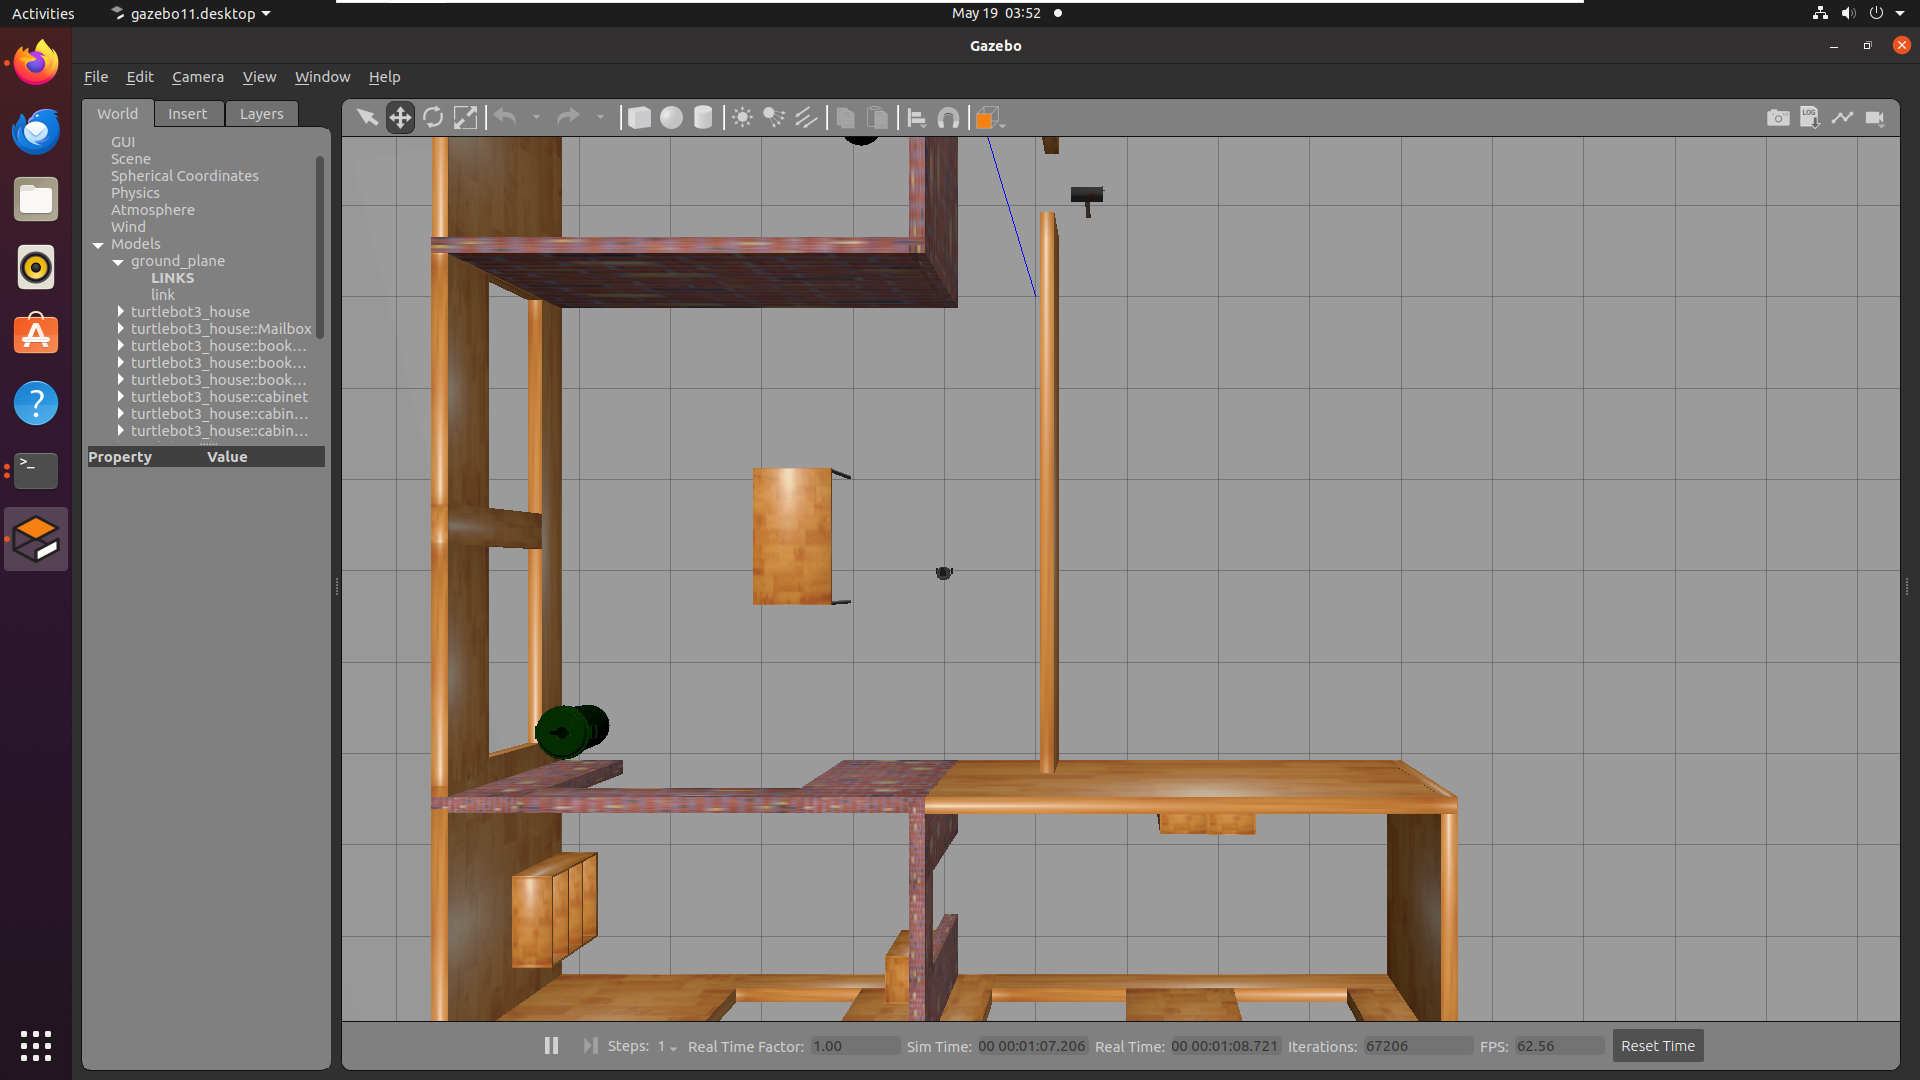
\includegraphics[width=0.75\linewidth]{imagenes/IntroROS - Gazebo House.png}
    \caption{Gazebo House}
\end{figure}

\section{Pruebas}

Para comprobar el correcto funcionamiento, se deciden probar una serie de mensajes ROS básicos que permiten mover el TurtleBot, recibir su posición y orientación, y por último recibir los datos del \textit{lidar}.

Para ello en la \textit{Command Window} de MATLAB introducimos lo siguiente:

\begin{lstlisting}[basicstyle=\scriptsize]
>> ipaddress = "http://192.168.197.128:11311";
>> rosinit(ipaddress)
\end{lstlisting}

Esto inicializará ROS, conectándose al TurtleBot que estamos simulando en Gazebo en la máquina virtual.

\subsection{Velocidad}

El mensaje tipo `/cmd\_vel' en ROS se utiliza para enviar comandos de velocidad al robot, especificando tanto la velocidad lineal como la angular que el robot debe seguir. Este mensaje, que suele ser publicado por nodos de control o de navegación, contiene información sobre la velocidad deseada en el espacio tridimensional, aunque comúnmente se utiliza en planos bidimensionales (velocidad lineal en los ejes x e y y velocidad angular alrededor del eje z).

\begin{lstlisting}[basicstyle=\scriptsize]
>> velocity = 0.1;
>> robotCmd = rospublisher("/cmd_vel","DataFormat","struct") ;
>> velMsg = rosmessage(robotCmd);
>> velMsg.Linear.X = velocity;
>> send(robotCmd,velMsg)
>> pause(4);
>> velMsg.Linear.X = 0;
>> send(robotCmd,velMsg)
\end{lstlisting}

\subsection{Posición}

El mensaje tipo `/odom' en ROS se utiliza para transmitir la información de odometría del robot, proporcionando datos esenciales sobre su posición y velocidad en el espacio. Este mensaje incluye la posición y orientación en coordenadas 3D del robot y su velocidad lineal y angular. Esta información permite implementar algoritmos de control y planificación del movimiento del robot.

\begin{lstlisting}[basicstyle=\scriptsize]
>> odomSub = rossubscriber("/odom","DataFormat","struct");
>> odomMsg = receive(odomSub,3);
>> pose = odomMsg.Pose.Pose;
x = pose.Position.X;
y = pose.Position.Y;
z = pose.Position.Z;
>> [x y z]

ans =

   -3.0002    1.0011   -0.0010
\end{lstlisting}

\subsection{Lidar}

El mensaje tipo `/scan' en ROS se utiliza para transmitir datos de sensores LiDAR. Este mensaje contiene información sobre la distancia medida a obstáculos en el entorno del robot, distribuida en un conjunto de ángulos. Los datos incluyen la distancia mínima y máxima detectada, el ángulo de inicio y final de escaneo, la resolución angular, y las intensidades de los retornos del láser si están disponibles. Estos datos son cruciales para tareas de navegación, mapeo y evitar obstáculos, ya que permiten que el robot perciba y responda de manera efectiva a su entorno.

\begin{lstlisting}[basicstyle=\scriptsize]
>> lidarSub = rossubscriber("/scan","DataFormat","struct");
>> scanMsg = receive(lidarSub);
>> rosPlot(scanMsg)
\end{lstlisting}

\begin{figure}[H]
    \centering
    \begin{subfigure}[c]{0.45\textwidth}
         \centering
         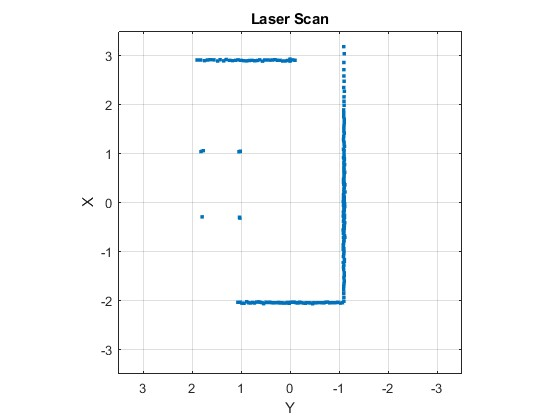
\includegraphics[width=\textwidth]{imagenes/Figura Lidar.jpg}
         \caption{Matlab}
     \end{subfigure}
     \hfill
     \begin{subfigure}[c]{0.45\textwidth}
         \centering
         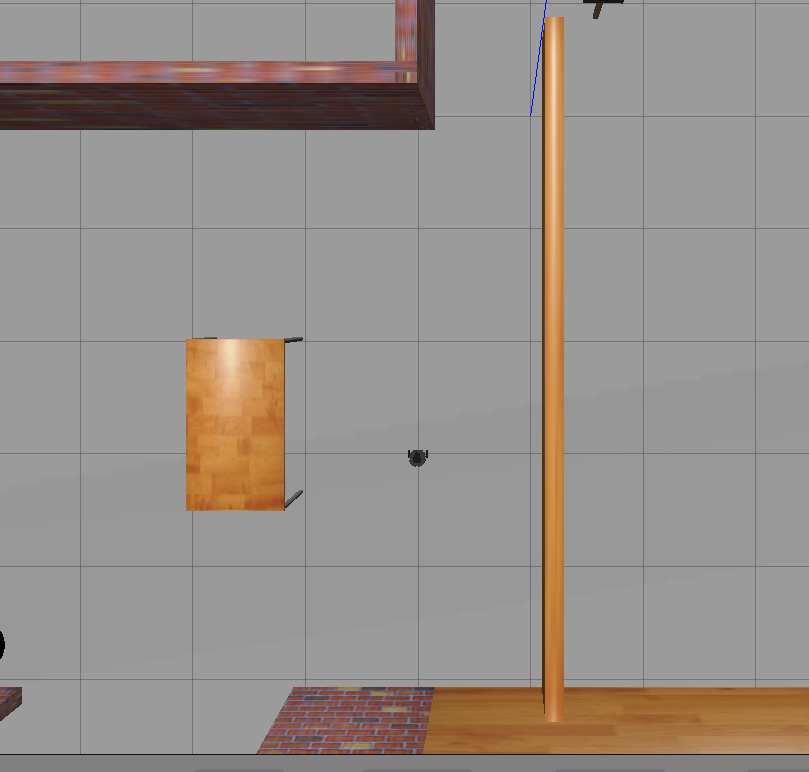
\includegraphics[width=\textwidth]{imagenes/Realidad Lidar.png}
         \caption{Gazebo}
     \end{subfigure}
    \caption{Comparación datos lidar y simulador.}
\end{figure}

%\blankpage